\documentclass[final,12pt]{article}    
%%%%%%%%%%%%%%%%%%%%%%%%%%%%%%%%%%%%%%%%%%%%%%%%%%%%%%%%%%%%%
%
%  include packages
%
\usepackage{times}
\usepackage{ifthen}
\usepackage{graphics}
\usepackage{graphicx}
\usepackage{color}
\usepackage{shadow}
\usepackage{makeidx}
\makeindex
%%%%%%%%%%%%%%%%%%%%%%%%%%%%%%%%%%%%%%%%%%%%%%%%%%%%%%%%%%%%%
%
%  if private=false certain descriptions are excluded using
%  the \ifthenelse expression
%
\newboolean{private}\setboolean{private}{true}
\newboolean{qmmm}\setboolean{qmmm}{true}
%%%%%%%%%%%%%%%%%%%%%%%%%%%%%%%%%%%%%%%%%%%%%%%%%%%%%%%%%%%%%
%
%  define commands
%
\newcommand{\block}[1]{\subsubsection[#1]{\shabox{\bf #1}}}
%
\newcommand{\brules}[1]{
\makebox[1in][l]{Rules:}\parbox[t]{110mm}{#1}\hfill\break\hfill}
%
\newcommand{\bdescr}[1]{
\makebox[1in][l]{Description:}\parbox[t]{110mm}{#1}\hfill\break}
%
%\newcommand{\key}[1]{\hfill\break
%\makebox[1in][l]{Keyword:}\parbox[t]{110mm}{{\bf #1}}\hfill\break}
%
\newcommand{\key}[1]{\hfill\break \makebox[1.5in][l]{\bf #1}\hfill\break}
%
%\newcommand{\vdescr}[1]{
%\makebox[1in][l]{}\parbox[t]{110mm}{#1}\hfill\break}
%
\newcommand{\vdescr}[1]{\makebox[1in][l]{}\parbox[t]{110mm}{#1}\hfill\break}
%
\newcommand{\vformat}[1]{
\makebox[1in][l]{}\parbox[t]{110mm}{\makebox[1in][l]{Type:}\parbox[t]{2.7in}{#1}}
\hfill\break}
%
\newcommand{\vrules}[1]{
\makebox[1in][l]{}\parbox[t]{110mm}{\makebox[1in][l]{Rules:}\parbox[t]{2.7in}{#1}}
\hfill\break}
%
\newcommand{\vdefault}[1]{
\makebox[1in][l]{}\parbox[t]{110mm}
{\makebox[1in][l]{Default:}\parbox[t]{2.7in}{#1}}
\hfill\break}
%
\newcommand{\mbax}[1]{#1}
%============================================================
%%%%%%%%%%%%%%%%%%%%%%%%%%%%%%%%%%%%%%%%%%%%%%%%%%%%%%%%%%%%%
%
% prepare titlepage
%
\title{{\bfseries\Huge 
    \hrulefill\\
    \hrulefill History Report for the \hrulefill\\
    \hrulefill \hrulefill Projector Augmented Wave \hrulefill\\
    \hrulefill Method \hrulefill\\}
    \medskip{\LARGE Version 2.0}\\
%\thanks{Peter~E.~Bl\"ochl, Clausthal University of Technology (2003)}\\   
%\resizebox{!}{9.0cm}{\includegraphics[10mm,15mm][90mm,110mm]{big.eps}}
\resizebox{!}{9.0cm}{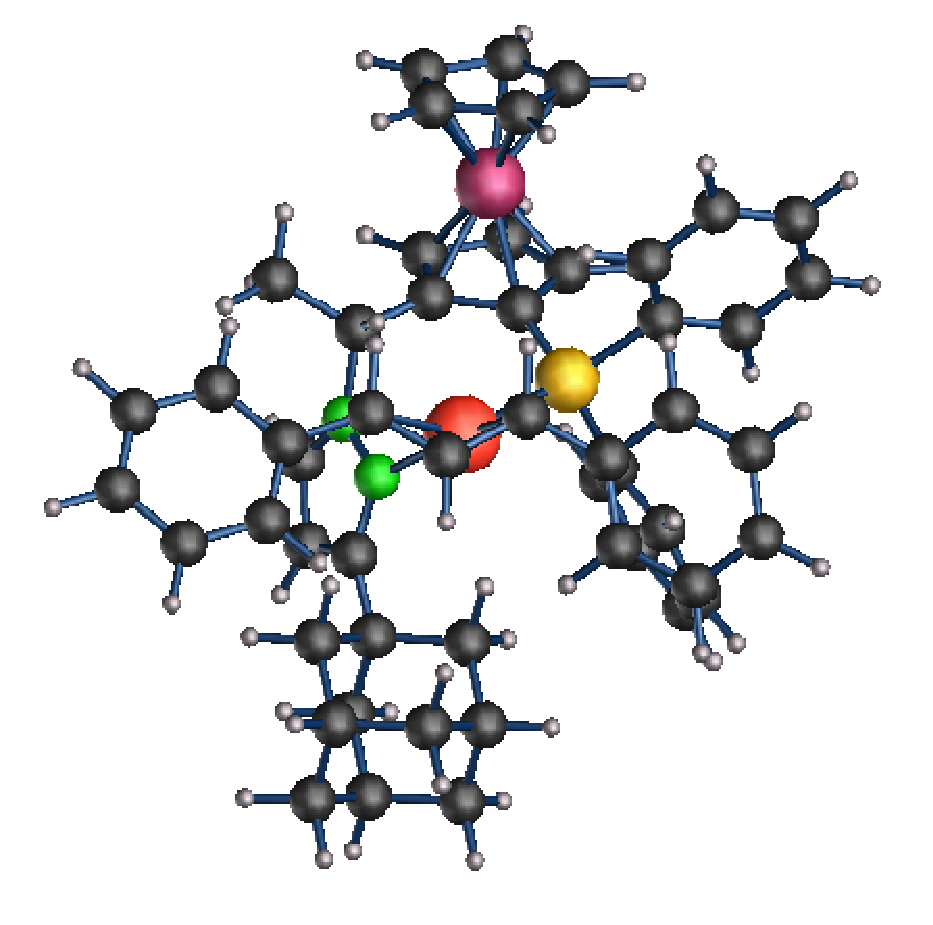
\includegraphics{Figs/big.eps}}
}
\date{\hrulefill\\Peter~E.~Bl\"ochl, Clausthal University of Technology\\(\today)}

\begin{document}          
\maketitle   
%
\noindent            
\setcounter{page}{1}
\footnote{The title picture shows the a chiral Pd complex with P,N ligands, a
  highly enantio-selective catalyst for allylic amination
  \cite{bloechl96_organometallics15_4125}.}
\newpage
\tableofcontents
%==========================================================================
\newpage
\setcounter{page}{1}
\section{Changes}
%==========================================================================
\subsection{28.Dec.06}

The Brillouin zone integration has been reworked substantially. 

The k-point grid can now be determined by a real space cutoff specified with
\verb+!STUCTURE!kPOINT:R+. This value specifies how fine the k-point grid is
chosen. The k-point grid corresponds to a supercell chosen so large that
real space points related by translational symmetry are separated at least by
the real space cutoff. 

Using the option \verb+STRUCTURE!KPOINTS:SHIFT+, the Monkhorst-Pack k-point
grid can now be shifted away from the $\Gamma$-point. Apparently this shift
improves the k-point convergence substantially. A shift of (1,1,1) is
recommended for crystals. The option may also improve the convergence with
cell-size for isolated molecules. However that needs to be tested.

In the block \verb+!CONTROL!MERMIN+ the option of quasi-adiabatic treatment of
the occupations is provided. A new set of energy levels is introduced that
approaches the Kohn Sham levels in a retarded fashion. The occupations are
optimized in each time step for this set of occupations. This option is
recommended for static calculations. It does not lead to an energy conserving
dynamics, because it is not a true adiabatic implementation.

As one of the quasi-adiabatic options the improved tetrahedron
method\cite{bloechl94_prb49_16223} has been included. Unlike the Mermin
functional\cite{mermin65_pr137_A1441}, this method does not require finite
temperatures. It is the recommended method for static calculations of metals.

In the printout the occupations are compared with those obtained from the
current energy eigenvalues. An estimate for the error in the energy is given
together with the maximum deviation of the occupations. 

\subsection{Jan. 11, 2007}

LDA+U option of Christian Walther implemented into main code. Some changes
have been made in this course. therefore testing will be required.

\subsection{Jan. 30, 2007}

COSMO can write an input file for COSMOTHERM.

\subsection{Feb. 25, 2007}

Rewrite of the linear algebra routines in paw_library.f90. Test routines have been 
included for the new routines. They are called by ``call lib\$test()''
Library specific driver routines are used, which distangles different libraries.
Has not been tested for ESSL library. Version has been checked into 
devel_blo/devel version 562.

\subsection{Feb 25.2007}

change in linkedlist\$existd. If a the nth data are searched true was
only returned, if nth was the total number NUM of data in the list. It has
been changed so, that the number NUM of elements in the list must be equal
or larger than nth.

\subsection{Apr 12. 2007}

The approximate hybrid functional has been included into the ldaplusu object.

\subsection{Apr 14. 2007}

Bugfix for plotting electrostatic potential. Symptom: The potential oscillated strongly.
Cause: POTSHIFT, an additive shift for the potential was added to all Fourier components 
of the potential instead of its real space values.

\subsection{Apr 14. 2007}

Bugfix in paw_library.f90. plans for fftw calls are now specified as integer(8). 
(integer(4), and integer did not work and produced a ``Speicherzugriffsfehler'' in the
 three dimensional fourier transform.)

\subsection{Apr 14. 2007}

Included tool paw_1davpot.x located in src/Tools/Wave. It uses the .wv
file produced by the !control!analyse!potential option and produces
the one-dimensional potential averaged over lattice planes. This tool
can be used to determine work functions and band offsets.

\newpage
\bibliographystyle{unsrt}
\bibliography{doc.bib}
\end{document}
\bye
%====================================================================
